	\section{Processi primari}

\subsection{Fornitura}
\label{sec:fornitura}
	
	\subsubsection{Scopo}
	Lo scopo di questa attività è quello di fornire il prodotto software proposto dall'azienda IKS S.r.l. e avente come committenti il Prof. Tullio Vardanega e il Prof. Riccardo Cardin.
	In questa sezione vengono trattate le norme, dalle più triviali alle più importanti, inerenti alla progettazione, lo sviluppo e la consegna del prodotto \emph{Havana}.
	Al fine di perseguire nel miglior modo questo traguardo intendiamo collaborare con i referenti dell'azienda, affrontando diversi punti fondamentali così da produrre un software completo e conforme alle richieste. Nello specifico è necessario:
    \begin{itemize}
	\item Stimare i costi del prodotto finale;
	\item Concordare la qualifica del prodotto;
	\item Determinare vincoli su processi e requisiti;
	\item Determinare aspetti fondamentali al fine di soddisfare la necessità del \gl{proponente}.
	\end{itemize}
	\subsubsection{Attività} 
		\paragraph{Studio di fattibilità} \Spazio
		Sono state organizzate diverse riunioni al fine di permettere ai membri del gruppo di scambiarsi opinioni sui capitolati proposti. 
		Abbiamo valutato i capitolati secondo diversi criteri:
		\begin{itemize}
			\item \textbf{Dominio tecnologico:} è stata presa in considerazione la conoscenza attuale delle tecnologie richieste per portare a termine i vari capitolati, in base anche ad esperienze passate avute con problemi simili;
			\item \textbf{Individuazione rischi:} sono state analizzate le varie difficoltà che si potrebbero incontrare durante la realizzazione dei vari capitolati considerando in modo particolare la mancanza di conoscenze adeguate relative alle tecnologie necessarie per realizzare i capitolati.
		\end{itemize}  \textit{}
	
	   \paragraph{Pianificazione} \Spazio
	   \label{sec:pianificazione}
	   Questa attività si divide in due rami i quali descrivono le scelte operative che il team segue per realizzare il prodotto finale così da rispettare dei fattori fondamentali per consegnare il sistema al richiedente. 
	   Nello specifico, viene trattato un piano per analizzare e gestire i fattori di rischio, una previsione di costo fornendo un budget per le varie voci di spesa, le attività da svolgere nel corso del progetto fornendo delle scadenze temporali precise e le convenzioni adottate dal team per revisionare le specifiche e testarle.
       Nel dettaglio:
       	       
	   \begin{itemize}
		\item \textbf{Piano di Progetto:} \Spazio
		Il \emph{Project Manager} affiancato dall'\emph{Amministratore} deve stilare un piano riportato in un documento che deve coprire le seguenti tematiche:
		\begin{itemize}
		\item \textbf{Analisi dei rischi:} si analizzano nel dettaglio i rischi che si potrebbero presentare durante lo svolgimento del progetto, determinando con quale probabilità potrebbero accadere e qual è il livello di gravità di ogni rischio;
		\item \textbf{Preventivo:} si stima, con una pianificazione, la quantità di lavoro necessaria per portare a termine ogni fase, in modo tale da riuscire a proporre un preventivo finale con il costo totale del progetto.
		\end{itemize}
		
		\item \textbf{Piano di Qualifica:} \Spazio
		Al \emph{\gl{verificatore}} è assegnato il compito di scegliere un metodo per la \gl{verifica} e \gl{validazione} del materiale realizzato dal team.
		Il documento deve coprire le seguenti tematiche:
		\begin{itemize}
		\item \textbf{Metodo di verifica:} vengono stabilite le procedure di controllo sulla qualità di \gl{processo} e di prodotto;
		\item \textbf{Metriche:} è necessario stabilire delle metriche oggettive per i documenti e i processi software;
		\item \textbf{Gestione della revisione:} si devono stabilire delle modalità per comunicare le anomalie e le procedure per controllare la qualità di processo;
		\item \textbf{Pianificazione test:} è necessario definire dettagliatamente le metodologie dei test a cui sarà sottoposto il progetto;
		\item \textbf{Resoconto attività verifica:} alla fine di ogni attività svolta si devono riportare le metriche relative e un resoconto sulla verifica effettuata.
		\end{itemize}
	\end{itemize}
	
\subsection{Sviluppo}
	\subsubsection{Scopo}
	Questo processo affronta le attività ed i compiti svolti dal gruppo al fine di sviluppare il software richiesto dal proponente. Per una corretta implementazione di tale processo è necessario:
	\begin{itemize}
		\item Realizzare un prodotto conforme alle richieste del proponente;
		\item Realizzare un prodotto conforme ai test di validazione e verifica;
		\item Fissare degli obiettivi di sviluppo.
	\end{itemize}
     Il processo di sviluppo si svolge secondo lo standard ISO/IEC 12207. È composto quindi, dalle seguenti attività:
     	\begin{itemize}
     	\item Analisi dei requisiti;
     	\item Progettazione;
     	\item Codifica.
     \end{itemize}
     
	

	\subsubsection{Attività}
		\paragraph{Analisi dei requisiti}
			\subparagraph{Scopo} \Spazio
			Lo scopo di questa analisi è quello di elencare nel modo più preciso possibile, tutti i requisiti del progetto. 
			I requisiti sono estrapolati da diverse fonti:
				\begin{itemize}
				\item Specifica del \gl{capitolato};
				\item Incontri tenuti direttamente con il proponente;
				\item Casi d'uso.
			\end{itemize}
		    Dopo aver svolto questo processo viene stilato in modo formale il documento \textit{Analisi dei Requisiti}.
		    Quest'ultimo è steso dagli \emph{Analisti} e contiene una lista dei requisiti e dei casi d'uso.
		    In questo modo sarà possibile effettuare e definire dei test di superamento del software. 

			\subparagraph{Casi d'uso} \Spazio
			Ogni caso d'uso è descritto dalla seguente struttura:
			\begin{itemize}
				\item Nome;
				\item Descrizione;
				\item Precondizione;
				\item Postcondizione;
				\item Inclusioni (se presenti);
				\item Estensioni (se presenti);
				\item Attori.
			\end{itemize}

			\subparagraph{Codice identificativo} \Spazio
			Ogni caso d'uso è identificato da un codice, ed è rappresentato nel seguente modo:
			
		    $$ \textbf{UC \{codice\_padre\}.\{codice\_figlio\}  } $$
			
			\begin{itemize}
				\item Le prime due lettere identificano che si tratta di un caso d'uso;
				\item Il codice padre è un numero univoco che identifica un caso d'uso;
				\item Il codice figlio è un numero progressivo che identifica i sottocasi;
			\end{itemize}
		Vi sono al massimo sei livelli di annidamento, la struttura numerica è completamente gerarchica.
		Consideriamo questo esempio:
		\begin{itemize}
			\item \textbf{UC1} Identifica il caso d'uso con numero univoco 1;
			\item \textbf{UC1.1} Identifica un nuovo livello figlio del numero 1;
			\item \textbf{UC1.1.1} Identifica un nuovo livello di annidamento gerarchicamente figlio del numero 1.1.
		\end{itemize}
	    Per ogni livello i numeri partono dal numero uno e non hanno limite massimo. 
			\subparagraph{Requisiti} \Spazio
			Ogni requisito è strutturato come segue:
			\begin{itemize}
				\item Nome;
				\item Tipo;
				\item Importanza;
				\item Stato implementazione;
				\item Fonti.
			\end{itemize}
			
			
			\subparagraph{Codice identificativo} \Spazio
			Ogni requisito è identificato da un codice, ed è rappresentato nel seguente modo:
			$$ \textbf{R \{importanza\}\{tipo\}\{numero\_vincolo\} } $$
			
			\begin{itemize}
				\item La R sta per requisito ed è presente in tutti i codici;
				\item Il primo valore rappresenza l'importanza: 0 se il requisito è obbligatorio, 1 se è desiderabile, 2 per gli opzionali;
				\item Il terzo valore indica il tipo: F per i requisiti funzionali, Q per quelli di qualità, P se prestazionale, V se di vincolo;
				\item L'ultimo numero indica il numero del vincolo. La struttura numerica di quest'ultimo rispetta le stesse regole dei Casi D'Uso.
			\end{itemize}
		
	        
		    
			\subparagraph{UML} \Spazio
			I diagrammi \gl{UML} devono essere realizzati usando la versione del linguaggio \textit{v2.0}
			
			
		\paragraph{Progettazione}
			\label{sec:progettazione}
			\subparagraph{Scopo}
			\Spazio
			L'attività di Progettazione ha lo scopo di definire e descrivere la progettazione ad alto livello dell'\gl{architettura} del prodotto richiesto e specificarla descrivendo la progettazione di dettaglio. \\
			Il responsabile di questa attività è il \emph{\gl{Progettista}} che, in funzione dei requisiti delineati nell'\textit{Analisi dei Requisiti}, è incaricato di discutere la \textit{Technology Baseline} tramite un \textit{Proof of Concept} che descrive le principali scelte tecnologiche e di discutere la \textit{Product Baseline} con un allegato tecnico che presenta le scelte architetturali del prodotto.
			Per fare ciò deve avere una profonda conoscenza dell'intero processo di sviluppo del software.
			Solo in questo modo può:
			\begin{itemize}
				\item progettare un software con le caratteristiche di qualità specificate nella fase di analisi e specifica dei requisiti;
				\item effettuare modifiche senza che la struttura del software già costruita debba essere messa nuovamente in discussione;
				\item soddisfare i requisiti di qualità fissati dal \gl{committente}.
			\end{itemize}
		
		
			\subparagraph{Technology baseline}
			\label{sec:tec}
			\Spazio
			Per la Revisione di Progettazione il progettista è tenuto a presentare e discutere in forma agile le scelte tecnologiche effettuate in finestre di opportunità che precedono la revisione: presenta le tecnologie, i \gl{framework} e le librerie selezionate per lo sviluppo del prodotto e ne dimostra l'adeguatezza e il grado di integrazione tramite un \textit{Proof of Concept} che sviluppa alcuni dei requisiti principali del progetto. Il \textit{PoC}, ovvero un prototipo eseguibile che dimostra ciò che il gruppo ha intenzione di realizzare, può rappresentare un punto di partenza per il progetto finale o soltanto un prototipo usa e getta.\\
			\textcolor{red}{---- Norme PoC?-----}\\
			Lo scopo delle attività che portano allo sviluppo della \textit{Technology Baseline} è permettere ai componenti del gruppo di prendere dimestichezza con le tecnologie che verranno utilizzate per lo sviluppo del software e permettere una migliore progettazione architetturale.

			\subparagraph{Product baseline}
			\label{sec:prod}
			\Spazio
			Per la Revisione di Qualifica, invece, il progettista è tenuto a presentare e discutere le scelte architetturali prese per il prodotto finale e dimostrando la coerenza con quanto scelto precedentemente nella \textit{Technology Baseline}.\\
			Per rappresentare al meglio le scelte prese si presenta un \emph{allegato tecnico} contenente:
				\begin{itemize}
					\item \textbf{Diagrammi UML:}
					essi forniscono una rappresentazione molto chiara e compatta dell'intera struttura dell'applicazione che si andrà ad analizzare. In particolare devono essere realizzati i seguenti diagrammi:
					\begin{itemize}
						\item \textbf{Diagrammi delle classi:} illustrano una collezione di elementi dichiarativi di un modello come classi e tipi, assieme ai loro contenuti e alle loro relazioni;
						\item \textbf{Diagrammi di sequenza:} descrivono una determinata sequenza di azioni dove tutte le scelte sono già effettuate. In pratica nel diagramma non compaiono scelte né flussi alternativi.
					\end{itemize}
					I diagrammi UML sono realizzati tramite il programma StarUML descritto nella sezione \ref{sec:StarUML};
					\item \textbf{\gl{Design Pattern}:}
					devono essere descritti i design pattern adottati all'interno dell'architettura del prodotto tramite descrizione e diagramma.
				\end{itemize}
		   La \textit{Product Baseline} è una milestone fondamentale dell'attività di progettazione e può contenere più o meno codice a seconda del grado di sviluppo del prodotto.\\
		   
		   Una volta svolta un'attenta analisi dell'architettura è compito del progettista offrire:
		   \begin{itemize}
		   	\item \textbf{Tracciamento delle componenti:}
		   	ogni requisito deve riferirsi al componente che lo soddisfa. Per fare ciò si utilizzerà SWEgo, un'applicazione web (descritta nella sezione \ref{sec:SWEgo}) utile nel tracciamento Use Case - Requisiti e nella generazione automatica dei diagrammi dei Casi d'Uso;
		   	\item \textbf{Test di integrazione:}
		   	i \emph{Progettisti} devono definire delle classi di verifica per verificare che i componenti del sistema funzionino nella maniera prevista.	
		   	\item \textbf{Tracciamento classi:}
		   	ogni requisito deve essere tracciato alle classi che lo soddisfano. Per fare ciò si utilizzerà SWEgo, un'applicazione web descritta nella sezione \ref{sec:SWEgo}.
		   	\item \textbf{Test di unità:}
		   	i \emph{Progettisti} devono definire i test di unità necessari per verificare che i componenti del sistema funzionino nel modo previsto.
		   \end{itemize}
		
		\paragraph{Codifica}
		\label{sec:codifica}
			\subparagraph{Scopo} \Spazio
			Questa attività ha come scopo l'effettiva implementazione del prodotto software richiesto. In questa fase dunque si concretizzano attraverso la codifica le funzionalità previste dai requisiti concordati.
			L'attività deve rispettare quando imposto dal documento \textit{Piano di Qualifica}.
			\subparagraph{Stile di codifica} \Spazio
			Al fine di garantire uniformità all'intera \gl{codebase}, ciascun membro del gruppo è obbligato a rispettare le seguenti norme:
			\begin{itemize}
			\item \textbf{Formattazione}: è richiesto l'uso di uno spazio (" ") ove possibile per rendere il codice di facile comprensione.
			Di seguito alcuni  esempi di buona e cattiva formattazione.
\begin{lstlisting}
int a=3; // BAD
int a = 3; // GOOD
int a = 3,b = 5; // BAD
int a = 3, b = 4; // GOOD

getFoo(a,b,c,d); // BAD
getFoo(a, b, c, d); // GOOD

if(a==5){ // BAD
if (a == 5) { // GOOD
\end{lstlisting}
			
			\item \textbf{Indentazione:} vengono utilizzati quattro spazi. L'\gl{IDE} utilizzato deve essere adeguatamente impostato per l'inserimento automatico di quattro spazi. Inoltre non sono permessi spazi bianchi o tabulazioni a fine riga;
			
			\item \textbf{Lunghezza linee di codice:} una riga di codice non deve superare i 100 caratteri, in caso contrario spezzare la riga di codice andando a capo;
			
			\item \textbf{Nomi:} i nomi delle funzioni e delle variabili devono essere significativi e devono cominciare con la lettera minuscola e seguire la convenzione camelCase. I nomi delle classi devono avere la prima lettera maiuscola mentre i nomi delle costanti devono essere scritti interamente in maiuscolo;
\begin{lstlisting}
var foo; // BAD
var profiledata // BAD
var profileData // GOOD
\end{lstlisting}
			
			\item \textbf{Lingua:} i nomi delle variabili i metodi le funzioni e i commenti vanno scritti in inglese;
			
			\item \textbf{Lunghezza metodi e funzioni:} il corpo dei metodi e delle funzioni non deve superare le 40 linee e i due gradi di indentazione. Se si superano tali limiti è un chiaro segno che la funzione/metodo necessita di essere riformattata in più funzioni. Gli unici metodi o funzioni ai quali è permesso ignorare questa norma sono quelli che contengono una componente logica troppo complicata per poter essere ulteriormente suddivisa in altri metodi o funzioni;
			
			\item \textbf{Numero di parametri per funzione:} una funzione non deve avere più di otto parametri;
			
			\item \textbf{Strutture di controllo:} le parentesi graffe per i costrutti che le prevedono devono essere sulle stessa linea del costrutto stesso. È prevista l'omissione delle graffe soltanto quando il corpo della struttura è di una sola riga;
\begin{lstlisting}
if (...) { // GOOD
	// CODICE
} else {
	// CODICE
}


if (...) // BAD
{
 	// CODE
}
else 
{
	// CODE
}

\end{lstlisting}
			\item \textbf{If annidati:} non sono ammessi più di due if annidati in modo da non compromettere la leggibilità del codice;
			\item \textbf{Numero condizioni per if: } non sono ammesse più di tre condizioni per If, in caso contrario è necessario raggruppare le condizioni in eccesso in funzioni con nomi che iniziano con la clausola "if";
\begin{lstlisting}
function isEven() { /*   */}

if (condizione && condizione && isEven()) { /*  */}

\end{lstlisting}

			\item \textbf{Commenti:} i commenti devono essere esaustivi e non prolissi in modo da aiutare il lettore a comprendere al meglio ciò che si sta leggendo. I commenti devono essere scritti in italiano.
			
			È inoltre consentito l'utilizzo di particolari tipi di commento con lo scopo di aiutare la stesura del codice. Vi sono:
			\begin{itemize}
				\item \textbf{TODO:} soluzione temporanee, memento di ogni tipo o zone che necessitano di un'implementazione.
				\begin{lstlisting}
// TODO: soluzione temporanea
// TODO: scrivere la query
				\end{lstlisting}
				
				\item \textbf{HOW:} per segnalare che non si ha capito l'implementazione o il funzionamento di una porzione di codice e che si necessita di uno studio più approfondito;
				\begin{lstlisting}
// HOW: da studiare il funzionamento della funzione f() usata
				\end{lstlisting}
				
				\item \textbf{FIX:} quando una particolare implementazione necessita di essere riparata o sistemata.
				\begin{lstlisting}
// FIX: funziona solo con la versione 3.0 di \gl{Internet Explorer}
				\end{lstlisting}
			\end{itemize}
			Questi commenti vanno scritti tutti in maiuscolo e seguiti da due punti (:), questa sintassi favorisce la loro individuazione da particolari \gl{tool} che ne permettono una consultazione agevolata.
			
			\end{itemize}
			\subparagraph{Intestazione} \Spazio
			Ogni \gl{file} contenente codice sorgente deve avere la seguente intestazione:
			\begin{lstlisting}
/*

* File : nome file
* Versione : versione file
* Tipo : tipo file
* Data : data di creazione
* Autore : nome autore 
* E-mail : email autore 
*
* License : tipo licenza				
*				
* Avvertenze : lista avvertenze e limitazioni
*
* Descrizione: breve descrizione del contenuto del file
*
* Registro modifiche :
* Autore || Data || breve descrizione modifiche
*
*/
			\end{lstlisting}
			\subparagraph{Versionamento} \Spazio
			Il versionamento dei file segue la filosofia \gl{Change Significance}. La versione di un file è espressa secondo la notazione $$X.Y.Z$$ I valori sono ordinati per importanza decrescente, partendo da sinistra. L'aumento di un parametro comporta l'azzeramento di tutti i parametri alla sua destra. Ogni volta che un file viene modificato deve essere propriamente aggiornata anche la versione. Il parametro da incrementare è:
			\begin{itemize}
				\item \textbf{X:} 
					\begin{itemize}
						\item Parte da 0;
						\item Se sono stati introdotti dei \gl{major improvement}, l'incremento di questo numero significa che sono state aggiunte funzionalità importanti. E.g: aggiunta di nuove classi / moduli;
						\item Solo il \emph{Verificatore} più aggiornare questo numero
					\end{itemize}
				
				\item \textbf{Y:} 
					\begin{itemize}
						\item Parte da 0;
						\item Se sono stati introdotti dei \gl{minor improvement}, \gl{bugfix}. Va incrementato in caso di implementazione di funzionalità più piccole. E.g: aggiunti singoli metodi, interfacce
						\item Solo il \emph{Verificatore} più aggiornare questo numero
					\end{itemize}

				\item \textbf{Z:}
					\begin{itemize}
						\item Parte da 0
						\item se sono stati corretti \gl{typos}, introdotti errori nei commenti o risolti piccoli \gl{bug}
						\item il \emph{Programmatore} e il \emph{Verificatore} possono modificare questo numero
					\end{itemize}
			\end{itemize}
			I parametri X,Y e Z non hanno un limite superiore e possono raggiungere anche valori maggiori di 9.
			Quando un file raggiunge la versione 1.0.0 significa che sono state implementate le funzionalità obbligatorie e quindi si può cominciare a testare il codice.
			\subparagraph{Ricorsione} \Spazio
			È caldamente sconsigliato l'utilizzo di ricorsione, esistono però dei casi in cui la soluzione ricorsiva renda il problema triviale, in tal caso è richiesta la verifica di correttezza e di terminazione della ricorsione.
			
	\subsubsection{Strumenti}
		\paragraph{StarUML}
		\label{sec:StarUML}
		\Spazio
		StarUML è uno strumento di modellazione UML compatibile con gli standard UML 2.x che supporta 11 tipi di diagrammi, tra cui i diagrammi delle classi, dei package, di attività e di sequenza che ci interessano per la progettazione del nostro programma.
		
		\begin{figure}[h]
		\label{figuraStarUML}
		\centering 
		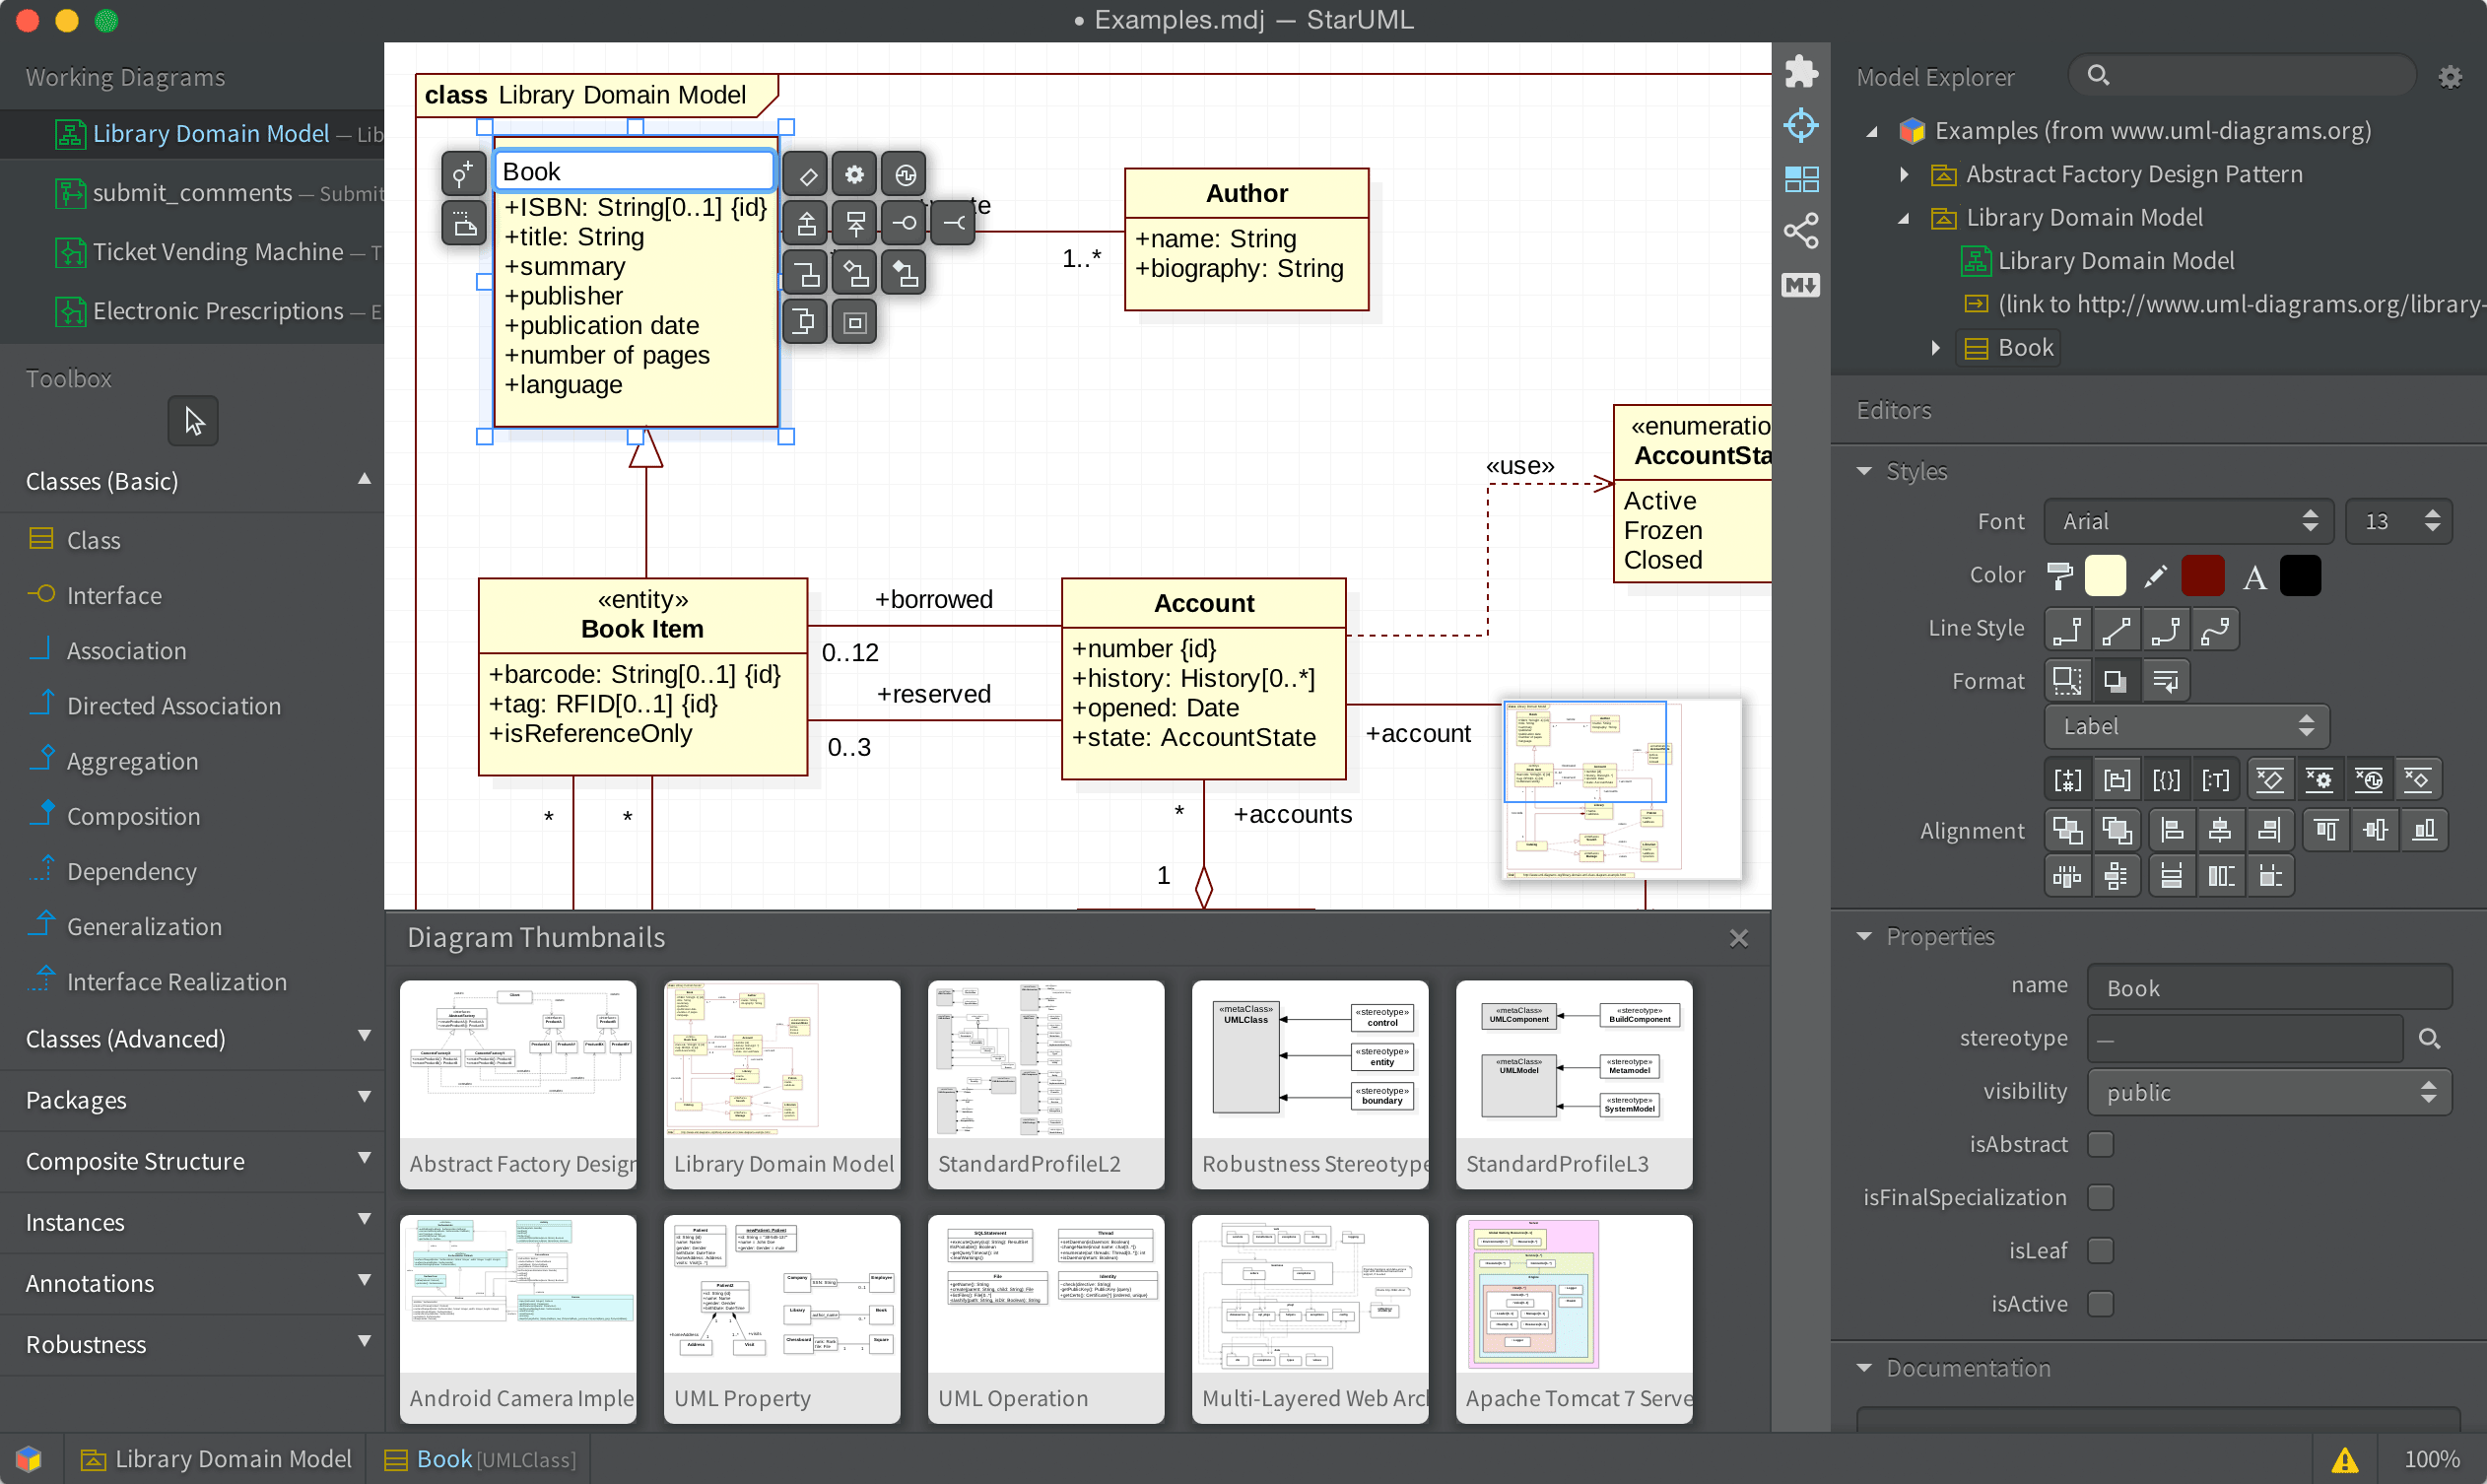
\includegraphics[width=1\textwidth]{images/starUML.png}
		\caption{Diagramma UML con StarUML} % descrizione
		\end{figure}

		
		\paragraph{SWEgo}
		\label {sec:SWEgo}
		\Spazio
		SWEgo è l'applicativo web scelto dal gruppo per il tracciamento dei requisiti. Offre molti servizi, come:
		\begin{itemize}
			\item \textbf{Tracciamento Use Case - requisiti:}
			tracciare un requisito serve a spiegare qual è l'origine di tale requisito e garantirne la necessità e la sufficienza. Il tracciamento è l'incontro tra i bisogni del proponente e dei requisiti;
			\item \textbf{Generazione automatica dei diagrammi dei Casi d'Uso utilizzando PlantUML:}
			SWEgo genera gli Use Case, dei diagrammi che esprimono un comportamento del sistema, offerto o desiderato, sulla base dei suoi risultati osservabili;
			\item \textbf{Visualizzazione grafici che indicano la copertura dei requisiti: }
			SWEgo permette di visualizzare le percentuali di copertura dei requisiti in tempo reale grazie a dei semplici grafici a torta.
		\end{itemize}
		\begin{figure}[H]
		\label{figuraSwego}
		\centering 
		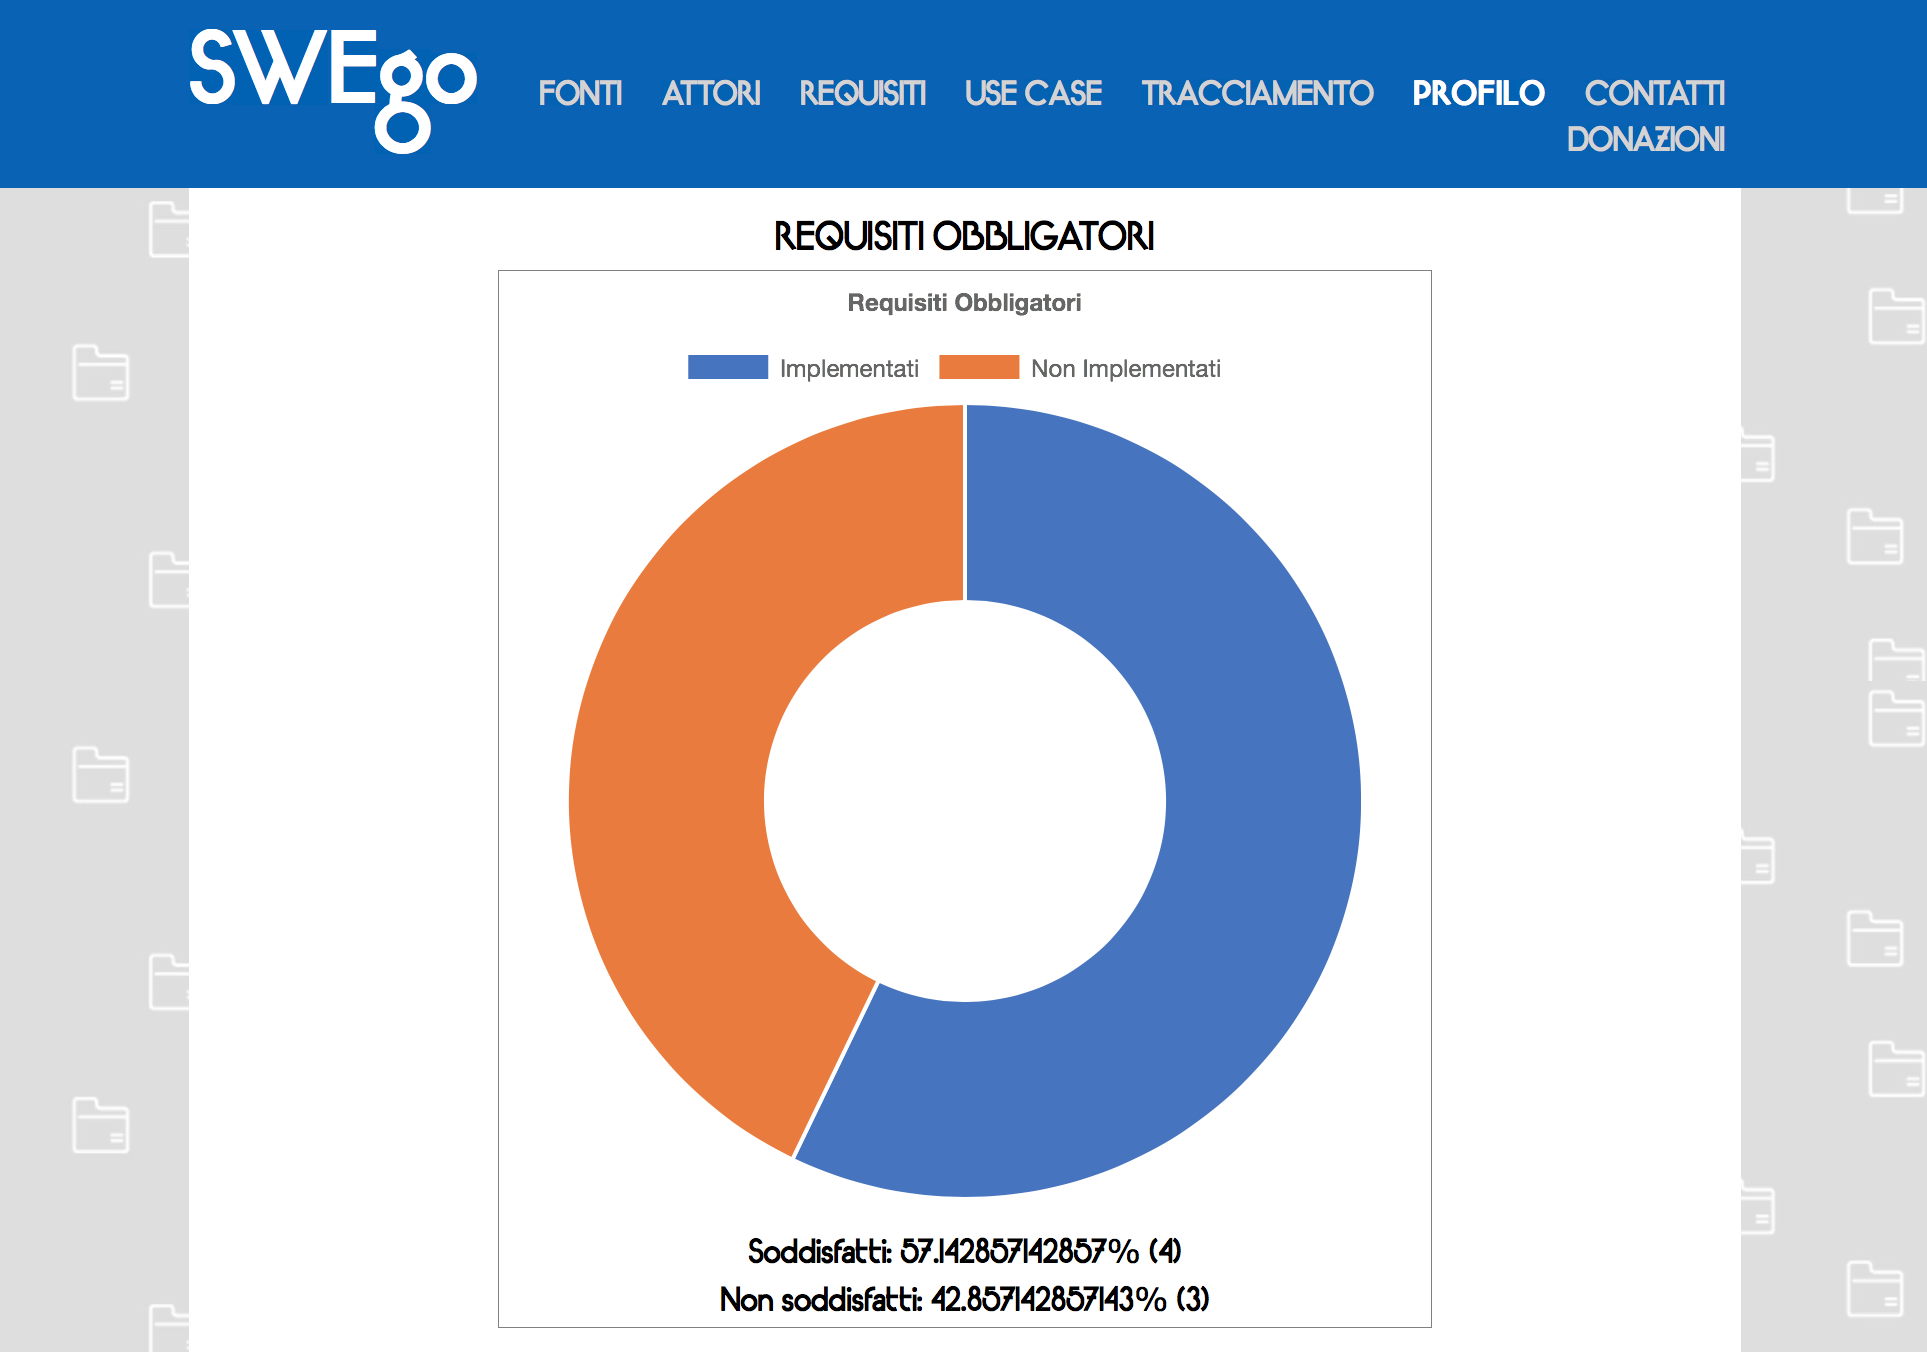
\includegraphics[width=1\textwidth]{images/swego1.png}
		\caption{Copertura requisiti con Swego} % descrizione
		\end{figure}
	
	\begin{figure}[H]
	\label{figuraSwego}
	\centering 
	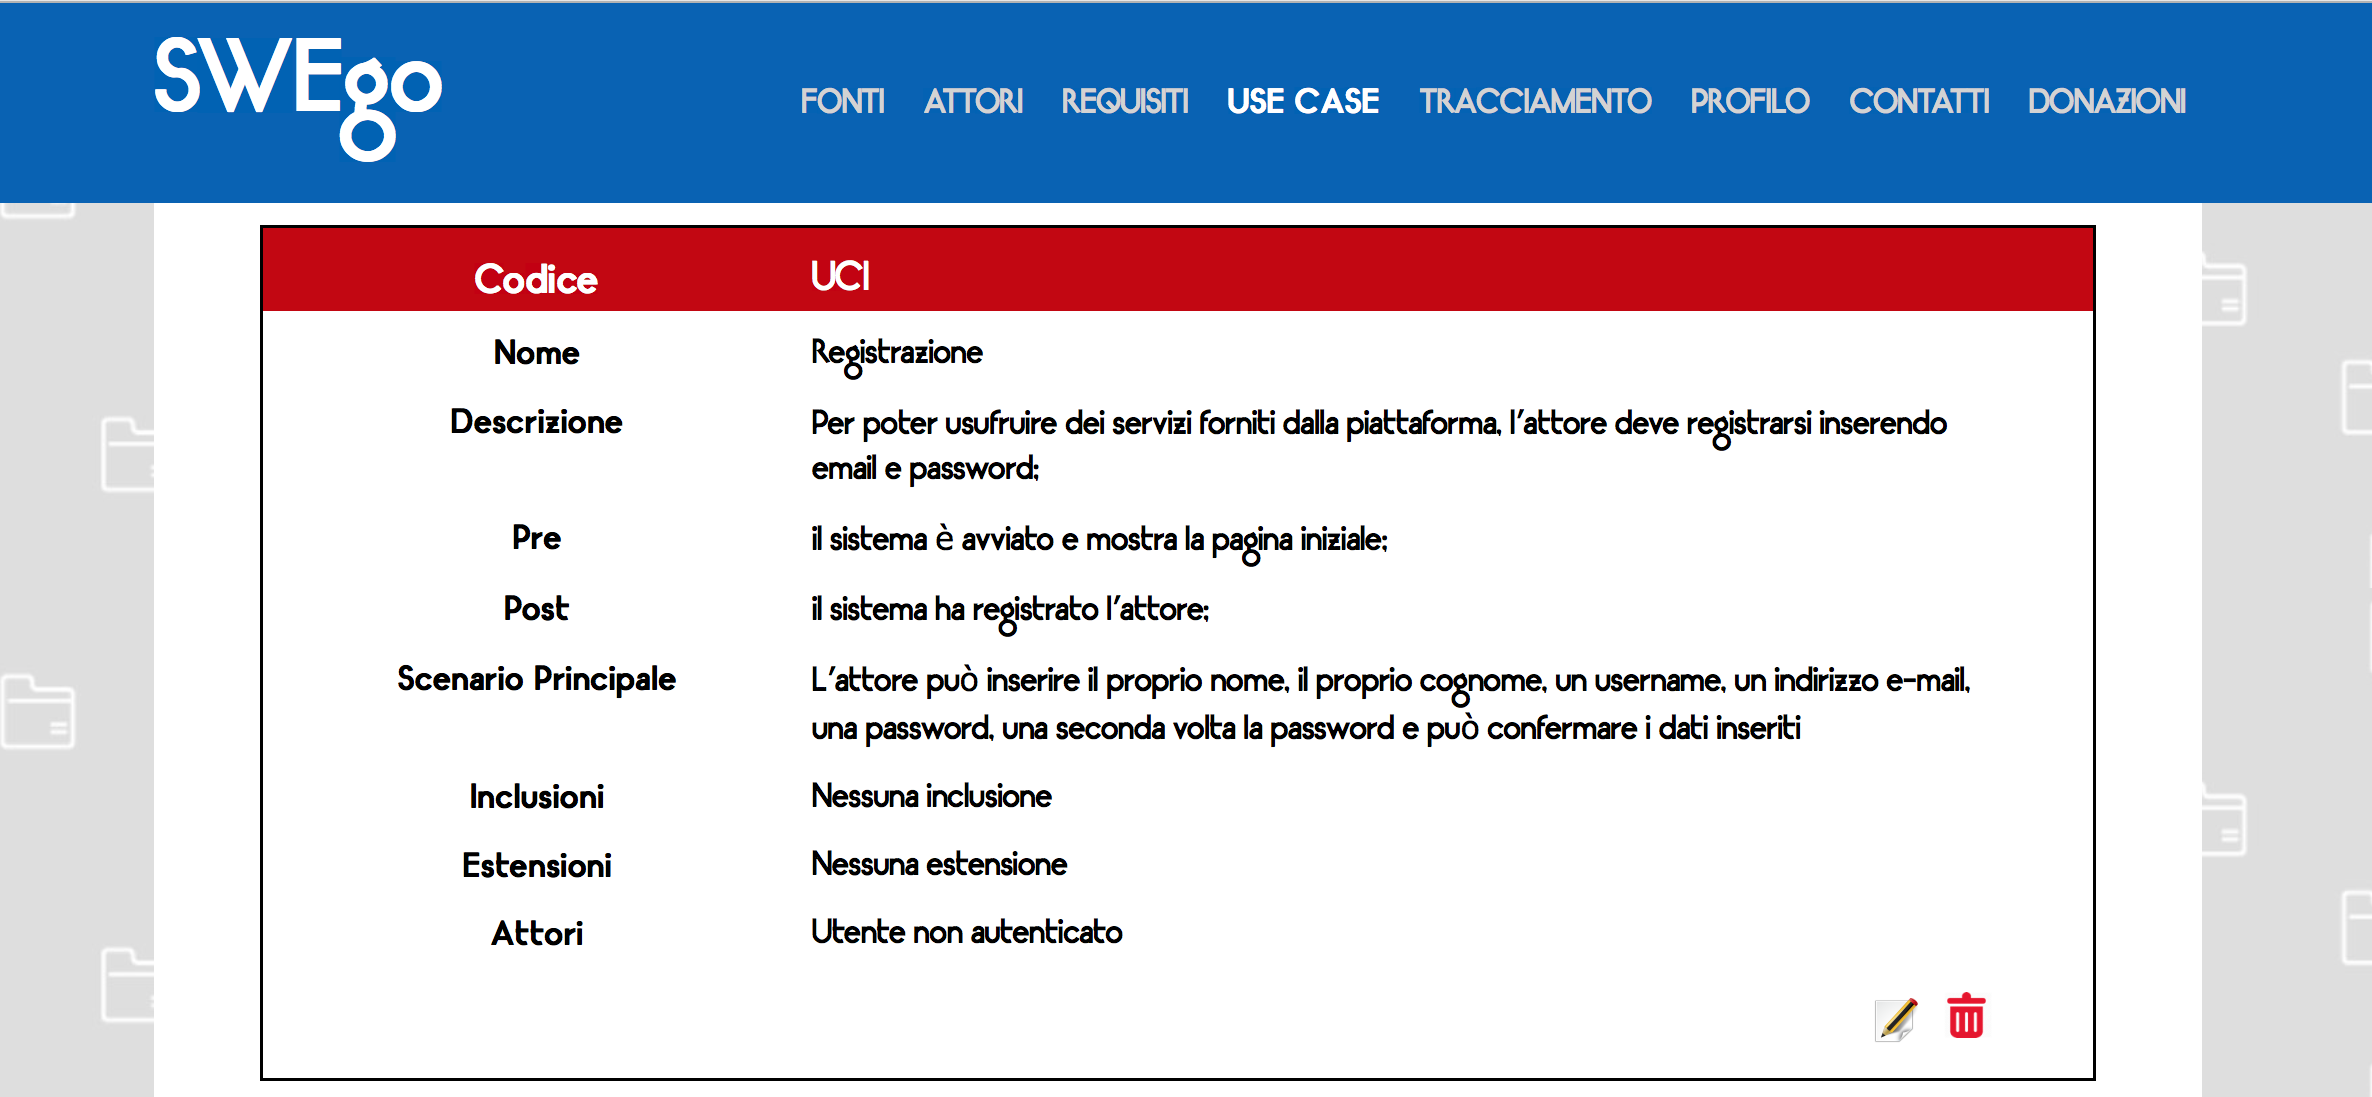
\includegraphics[width=1\textwidth]{images/swego2.png}
	\caption{Use Case con Swego} % descrizione
	\end{figure}


	
	\paragraph{Atom}
	\label{sec:Atom}
	\Spazio	
	Atom è un IDE di ultima generazione, sviluppato da \gl{GitHub}. È un \gl{editor} potente,
	\gl{crossplatform} e si integra perfettamente con tutte le tecnologie e strumenti che si utilizzano per lo sviluppo del prodotto. Infatti questo IDE mette a disposizione l'highlighting del codice per permettere una stesura ed una lettura agevolata. 
	Offre inoltre un vastissimo numero di plugin grazie al grande supporto della comunità \gl{open source} che lo sviluppa. Tra i plugin che il team utilizzerà vi è \gl{SonarJS}, che permette l'analisi statica del codice, questo tool infatti proviene dalla suite \gl{SonarQube} che SWEefty ha scelto come strumento principale per l'analisi statica del codice in quanto fornisce meccanismi avanzati per questo tipo di attività.
	
	\begin{figure}[H]
		\label{Atom}
		\centering 
		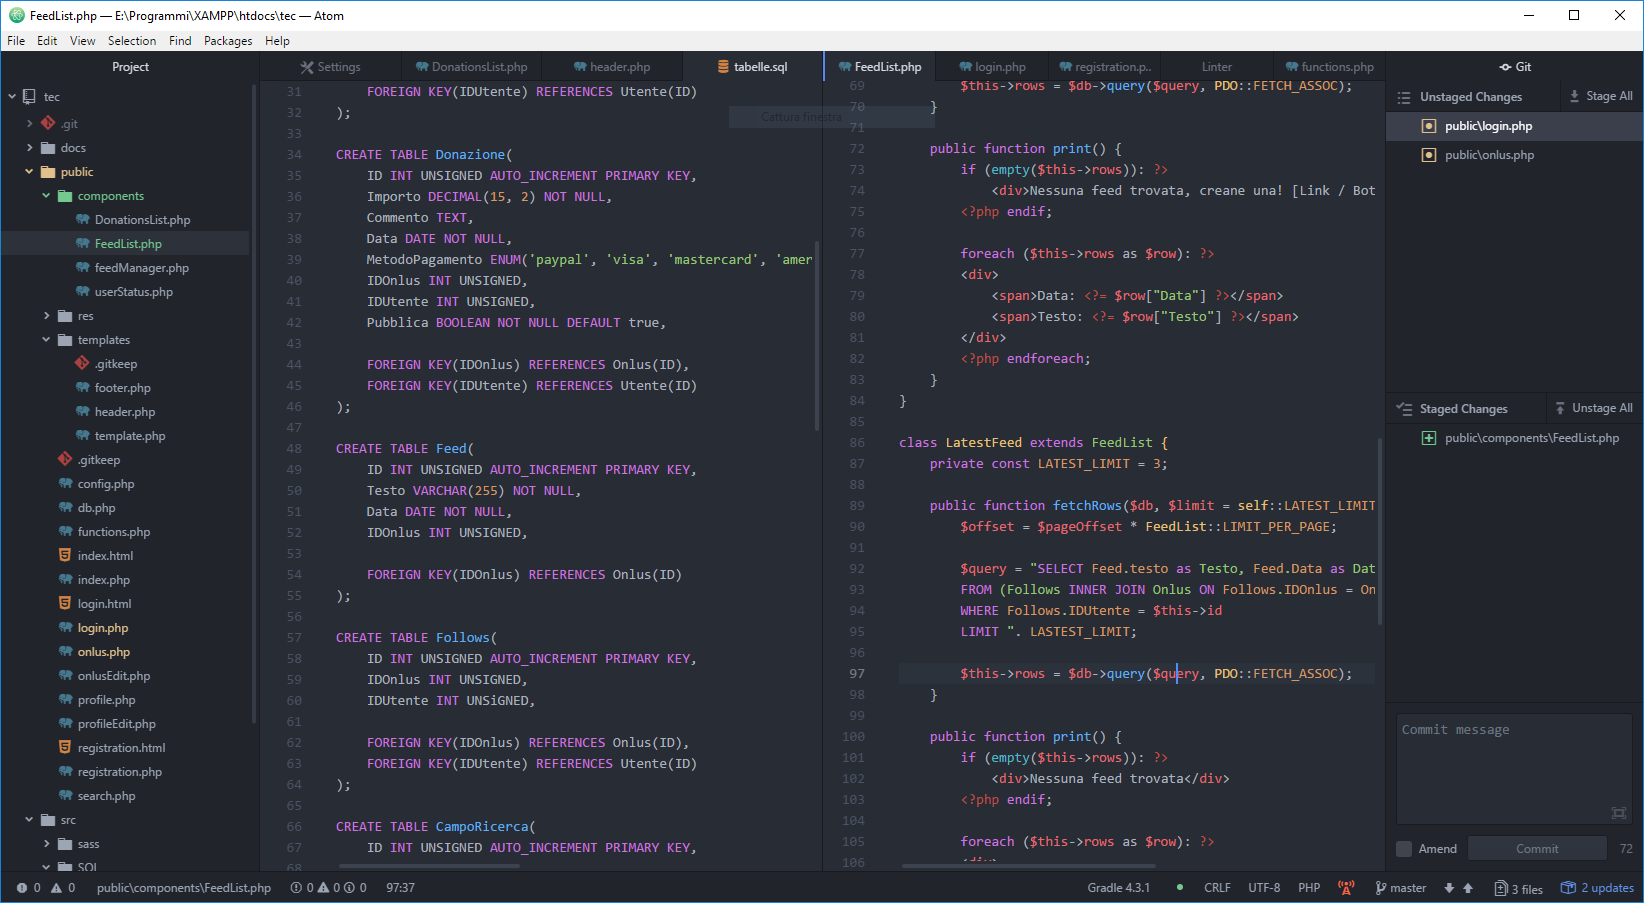
\includegraphics[width=1\textwidth]{images/atom.png}
		\caption{Interfaccia grafica di Atom per Windows} % descrizione
	\end{figure}
	
			
